\chapter{FPGA Implementation, Self-Test and Board Results}\label{ch:hw}

\section{System on the Kria KV260}

The detector runs on an AMD Kria KV260 board (Zynq UltraScale+ XCK26: four Arm Cortex-A53 cores and FPGA fabric).
In the final design (kit v6) the Arm cores only move raw samples; the front end and the classifier both run in the
fabric (Figure~\ref{fig:arch}).

\begin{figure}[H]
\centering
\resizebox{\textwidth}{!}{% SeizeLUT on the KV260 (kit v6): processing system (Arm) and programmable logic (fabric)
\begin{tikzpicture}[font=\scriptsize, >=stealth,
  blk/.style={draw, rounded corners=1.5pt, align=center, minimum height=5.2mm, inner sep=1.6pt, fill=white},
  grp/.style={draw, dashed, rounded corners=3pt, inner sep=3pt}]
  % Arm side
  \node[blk] (sens) at (0,0) {bte-EEG$\times$2, ECG,\\EMG, ACC, GYR};
  \node[blk, right=3mm of sens] (drv) {driver: raw samples\\$\to$ AXI4-Lite};
  \node[grp, fit=(drv), label={[font=\scriptsize\bfseries]above:Arm Cortex-A53 (PS)}] (ps) {};
  % fabric
  \node[blk, below=8mm of sens.south west, anchor=north west] (fe) {feature engine\\shift-add, 2,323 instr.\\38 features / s};
  \node[blk, right=2.5mm of fe] (cmp) {146\\comparators};
  \node[blk, right=2.5mm of cmp] (lut) {50 LUT6\\(DWN)};
  \node[blk, right=2.5mm of lut] (pop) {popcount\\score};
  \node[blk, right=2.5mm of pop] (alm) {decision,\\$k$-of-10 alarm};
  \node[blk, below=3.5mm of cmp] (rom) {BIST ROM\\255 + 769 vectors};
  \node[blk, below=3.5mm of lut, xshift=5mm] (fi) {fault injection\\(stuck-at, TT flip)};
  \node[blk, below=3.5mm of alm] (chk) {BIST check: score,\\decision, alarm};
  \node[blk, below=3.5mm of fe] (io) {alarm out: LEDs,\\buzzer, button};
  \node[grp, fit=(fe)(alm)(rom)(io)(chk), label={[font=\scriptsize\bfseries]below:programmable logic, 100 MHz, no multiplier}] (pl) {};
  \draw[->] (sens) -- (drv);
  \draw[->] (drv.south) |- ++(0,-3mm) -| (fe.north);
  \draw[->] (fe) -- (cmp);
  \draw[->] (cmp) -- (lut);
  \draw[->] (lut) -- (pop);
  \draw[->] (pop) -- (alm);
  \draw[->] (rom.north) -- (cmp.south);
  \draw[->] (fi.north -| lut.south) -- (lut.south);
  \draw[->] (alm.south) -- (chk.north);
\end{tikzpicture}
}
\caption{SeizeLUT on the Kria KV260. The fault-injection registers and the self-test let the device check that the
fabric still computes the validated classifier.}\label{fig:arch}
\end{figure}

\begin{itemize}
\item \textbf{Interface:} one AXI4-Lite slave at 100\,MHz with an 8-KB window: control and result registers, the
  feature registers, and the feature engine's register file at 0x1000.
\item \textbf{Classifier:} 146 threshold comparators, 50 LUT6, popcount score, frozen and programmable operating
  points, 10-of-10 alarm, latency 3 clock cycles.
\item \textbf{Test logic:} built-in self-test (BIST) with its vector ROM, fault-injection registers, read-back of
  all comparator bits and LUT outputs.
\item \textbf{Demo I/O:} PMOD outputs for an alarm LED, a buzzer, score LEDs and a heartbeat, and a debounced button.
\end{itemize}

\section{Front End in the Fabric}\label{sec:fe-engine}

A front end with dozens of filters would need many multipliers if built directly. Instead, a small microcoded
\emph{feature engine} computes the 38 features the classifier reads, one instruction at a time:

\begin{itemize}
\item one 40-bit adder and two 5-bit shifters; every filter coefficient is a sum of at most five signed powers of
  two, so a multiplication becomes a few shifted additions;
\item a register file (930 words) and a 2,323-instruction program in block RAM, 3 clock cycles per instruction;
\item four events: a 256-Hz biopotential sample, a 25-Hz motion sample, the end of a second, and the last window.
\end{itemize}

After each window the core copies the engine's 38 features into the classifier and classifies them automatically.

\begin{table}[H]
\centering\small
\caption{Verification of the feature engine.}\label{tab:fe-verif}
\begin{tabularx}{\textwidth}{@{}LP{58mm}@{}}
\toprule
\textbf{Check} & \textbf{Result}\\
\midrule
Program (instruction-level simulator) against the C front end, 10 recordings & all 431,960 windows equal (38 features)\\
Engine RTL fed sample by sample (Verilator), EEG-only and all-sensor recording & 4,278 windows, 0 mismatches\\
Whole core from raw samples through AXI (Verilator) & 4,278 windows: features, score, decision, alarm equal\\
On the KV260 board, 3 raw recordings & 9,214 windows, 0 feature and 0 output mismatches\\
Busy cycles per second of signal & at most 946,168 (simulation and board identical)\\
\bottomrule
\end{tabularx}
\end{table}

The engine needs under one million cycles per second of signal, so it keeps up with the sensors at 1\,MHz, a
hundredth of the board's clock.

\section{Hardware Cost}

\begin{table}[H]
\centering\small
\caption{Cost of the LUT-native classifiers on the XCK26 (Vivado 2026.1 out of context, 2.5-ns constraint,
vectorless power at 400\,MHz; Yosys \texttt{synth\_xilinx} as a second flow).}\label{tab:hwcost}
\begin{tabular}{@{}lrrrrrr@{}}
\toprule
\textbf{Model} & \textbf{LUTs} & \textbf{FFs} & \textbf{Fmax} & \textbf{Dyn. power} & \textbf{Yosys LUTs} & \textbf{Test F1}\\
\midrule
\textbf{DWN + distillation (ours)} & \textbf{398} & 454 & \textbf{468\,MHz} & \textbf{17\,mW} & 405 & 0.248\\
TreeLUT (5-bit leaves) & 2,677 & 1,461 & 294\,MHz & 88\,mW & 2,721 & 0.233\\
Logic-gate network & 5,249 & 2,208 & 154\,MHz & 523\,mW & 5,758 & 0.191\\
\bottomrule
\end{tabular}
\end{table}

\begin{table}[H]
\centering\small
\caption{Cost of the whole detector and of the KV260 design (Vivado 2026.1, user's build).}\label{tab:whole}
\begin{tabularx}{\textwidth}{@{}LP{70mm}@{}}
\toprule
\textbf{Part} & \textbf{Cost}\\
\midrule
Feature engine alone (out of context) & 804 LUTs, 101 FFs, 4.5 block RAMs, 0 DSP, 234\,MHz\\
Whole detector (feature engine + DWN) & \textbf{1,202 LUTs, no multiplier} (Yosys: 797 + 405, also 1,202)\\
Whole core in the design (with BIST, fault injection, debug, demo I/O) & 3,356 LUTs, 13.5 block RAMs\\
Full KV260 design & 3,796 LUTs (3.2\,\% of the device), 0 DSP; timing met at 100\,MHz (slack 3.5\,ns)\\
\bottomrule
\end{tabularx}
\end{table}

The DWN needs 6.7 times fewer LUTs than TreeLUT and 13.2 times fewer than the logic-gate network, and it is also the
fastest. Its thermometer comparators, not the network, take most of its cost.

\section{Self-Testing}

\paragraph{Fault model.} Every single fault in the part of the hardware the network adds: each of the $50 \times 64 =
3{,}200$ truth-table bits flipped (an upset in FPGA configuration memory) and each comparator and LUT output stuck at 0
or 1 (292 + 100): 3,592 faults.

\paragraph{Which faults matter.} Each fault was applied to all 31.4 million windows (8,714 hours) of the 96 training
patients. A fault is \emph{decision-relevant} if it changes at least one decision.

\paragraph{Test vectors.} The vectors were chosen from training windows to cover the rarely used truth-table entries
first (Table~\ref{tab:faults}, Figure~\ref{fig:faultcov}).

\begin{table}[H]
\centering\small
\caption{Single faults on the training data and the decision-relevant faults detected (\%) by three self-test vector
sets.}\label{tab:faults}
\begin{tabular}{@{}lrrrrrr@{}}
\toprule
\textbf{Fault} & \textbf{All} & \textbf{Decision} & \textbf{Alarm} & \textbf{Consecutive} & \textbf{Random} &
\textbf{Selected}\\
\midrule
truth-table bit flipped & 3,200 & 2,498 & 1,674 & 43.6 & 79.4 & \textbf{100.0}\\
comparator stuck at 0/1 & 292 & 292 & 289 & 94.5 & 100.0 & \textbf{100.0}\\
LUT output stuck at 0/1 & 100 & 100 & 100 & 100.0 & 100.0 & \textbf{100.0}\\
\midrule
\textbf{all} & 3,592 & 2,890 & 2,063 & 50.7 & 82.2 & \textbf{100.0}\\
\bottomrule
\end{tabular}
\end{table}

\begin{figure}[H]
\centering
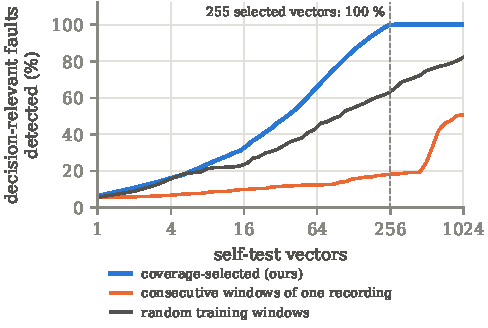
\includegraphics[width=0.75\textwidth]{figures/fault_coverage.pdf}
\caption{Decision-relevant faults detected by the first $m$ self-test vectors.}\label{fig:faultcov}
\end{figure}

The natural choice of a test, 1,024 consecutive recorded windows, detects only 50.7\,\% of the faults that change a
decision; the 255 selected windows detect all of them. The on-chip self-test runs 1,024 vectors in 1,028 clock cycles
(10.3\,\textmu s), so the device can test itself after every one-second window.

\section{Board Results}

The board runs Ubuntu 22.04 with Kria-PYNQ. One script (\texttt{run\_board\_tests.sh}) runs nine tests and saves all
numbers to a results file. Table~\ref{tab:board} gives the full campaign on our KV260.

\begin{table}[H]
\centering\small
\caption{Board test campaign on the KV260 (kit v6 bitstream, Vivado 2026.1).}\label{tab:board}
\begin{tabularx}{\textwidth}{@{}P{38mm}LP{22mm}@{}}
\toprule
\textbf{Step} & \textbf{Measured on the board} & \textbf{Result}\\
\midrule
1 Identity & core version 3, 38 features, 50 LUTs; bitstream loads in 4.4\,s & PASS\\
2 Self-test & 1,024 of 1,024 vectors correct in 1,028 cycles & PASS\\
3 Latency & 3 clock cycles (30\,ns) & PASS\\
4 Replay & all 431,960 windows of 10 recordings through the registers: 0 mismatches at both operating points;
  3.2\,\textmu s per window & PASS\\
5 Detection (10 recordings) & frozen point: 1 of 19 seizures, 0 false alarms in 120\,h; programmable point: 3 of 19,
  25 false alarms (equal to simulation) & reported\\
6 Power & 3.069\,W idle, 3.074\,W with the classifier fed one window per clock (difference within the sensor's
  noise) & reported\\
7 Front end on the Arm & 3 raw recordings: 0 feature and 0 output mismatches, 3,390--4,080 times faster than real
  time & PASS\\
8 Fault injection & all 3,592 faults injected: 0 hardware/software mismatches; all 2,890 decision-relevant faults
  detected; 88\,s & PASS\\
9 Whole detector in the fabric & 9,214 windows from raw samples: 0 feature and 0 output mismatches; engine busy
  for exactly the simulated cycles (787,615 / 787,521 / 946,168 per second); 102--124 times faster than real time &
  PASS\\
\bottomrule
\end{tabularx}
\end{table}

Step 5 covers only the 10 exported recordings of three test patients, as a check that the board reproduces the
software; the detection results on all 29 test patients are in Chapter~\ref{ch:results}. The first board run found one
software bug: the driver wrote ``soft reset'' and ``clear counters'' in the same register write, and the hardware
gives the reset priority, so the counters were not cleared. The driver now writes them separately (no rebuild).

\section{Live Demo}

Recorded test-patient signals stream second by second through the board, and a laptop browser shows every stage:
signals, features, comparator bits, LUT votes, score and alarm, with a check on every window that the FPGA equals the
software (Figure~\ref{fig:dashboard}). On the breadboard, the FPGA drives a red alarm LED (PMOD B1, 220\,$\Omega$) and
a buzzer through a BC547 transistor (PMOD B2, 1\,k$\Omega$). On the board the alarm fires during the seizure and the
LED and buzzer turn on.

\begin{figure}[H]
\centering
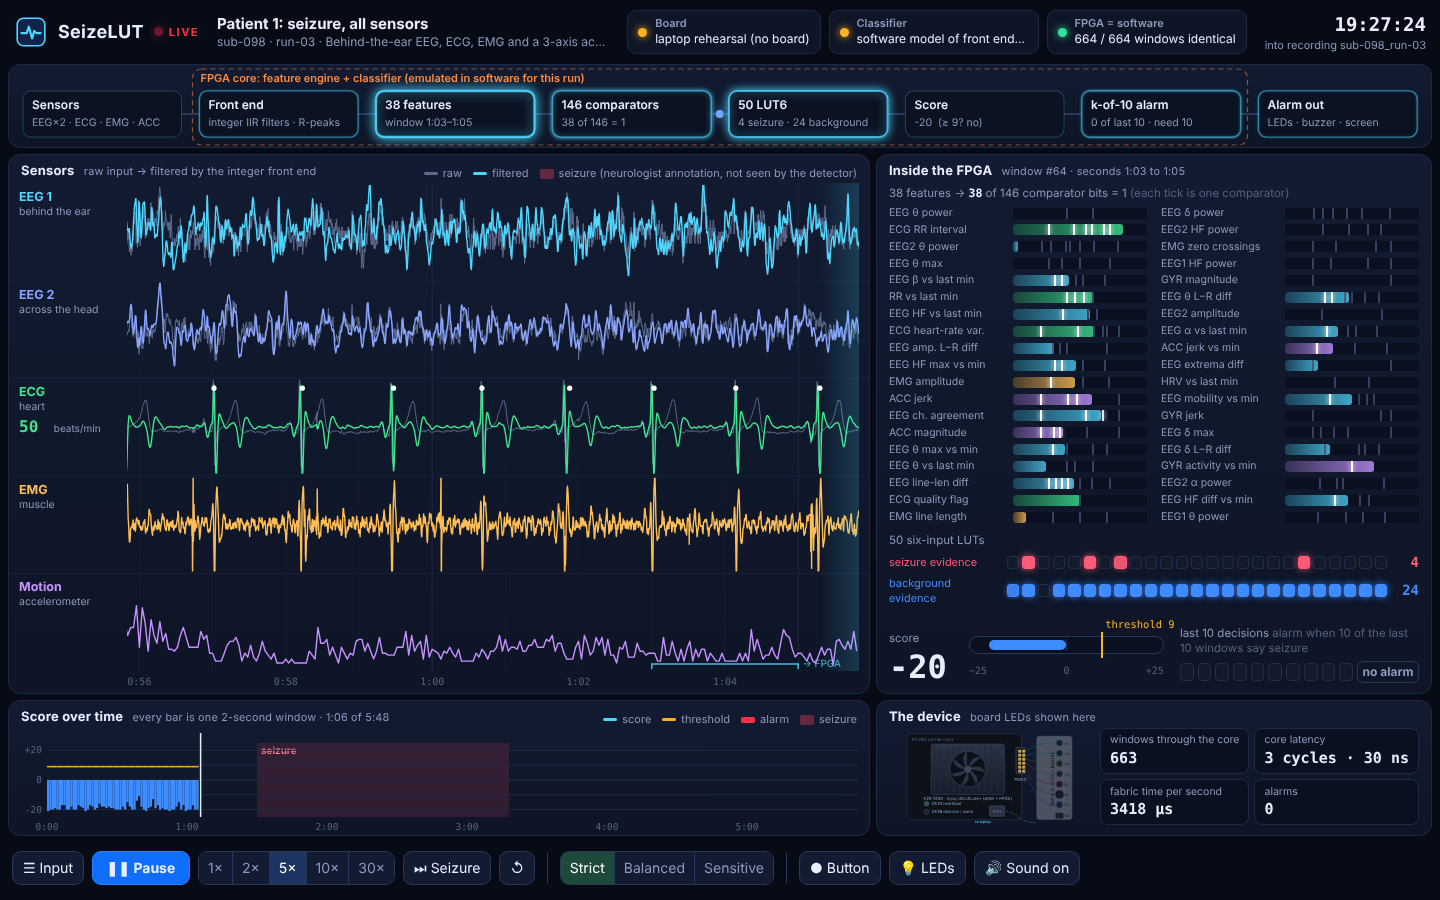
\includegraphics[width=\textwidth]{figures/dashboard_rehearsal.png}
\caption{Live dashboard (laptop rehearsal with the software model of the core; on the board the same page shows the
FPGA).}\label{fig:dashboard}
\end{figure}
